\section{The Metropolis-Hastings Algorithm}

\textit{Metropolis-Hastings algorithm} is one of the most used \textit{Markov Chain Monte Carlo}(MCMC) algorithm.
The \textit{Metropolis algorithm} was first introduced by Nicholas Metropolis in 1953 in his paper entitled \textit{"Equation of State Calculations by Fast Computing Machines"}, with Arianna W. Rosenbluth, Marshall Rosenbluth, Augusta H. Teller and Edward Teller.
Arianna Rosenbluth wrote the first full implementation of Metropolis Algorithm for  \textit{Mathematical Analyzer Numerical Integrator and Automatic Computer Model I}(MANIAC 1) which was an early computer built under the direction of Nicholas Metropolis at the Los Alamos Scientific Laboratory.

\begin{figure}[H]
	\centering
	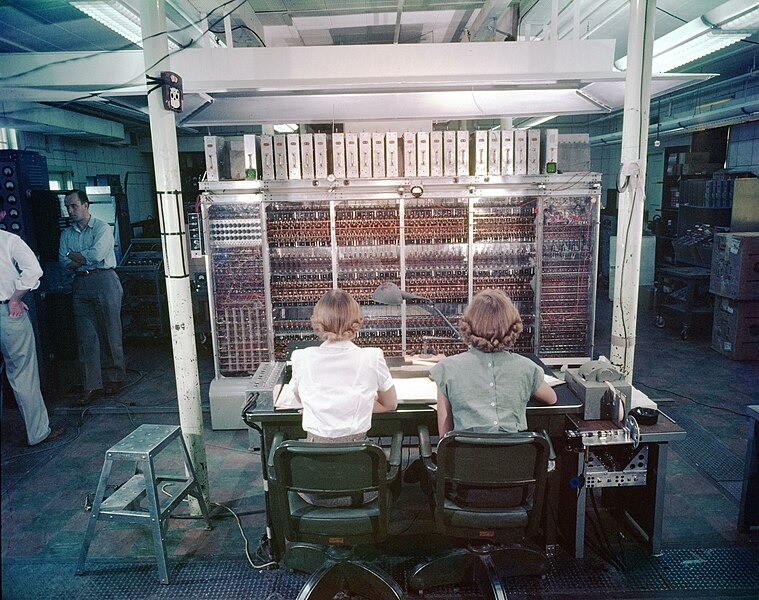
\includegraphics[width=0.4\textwidth]{Operators_in_front_of_the_MANIAC.jpg}
	\caption{MANIAC 1 one of the early computer.}
	\label{MANIAC}
\end{figure}

For may years this algorithm is was simply known as \textit{Metropolis Algorithm}, later in 1970 W.K. Hastings introduce more general version of this algorithm in his paper \textit{"Monte Carlo Sampling Methods Using Markov Chains and Their Applications"}. This generalized Metropolis algorithm is known as \textit{Metropolis-Hastings algorithm}(MH algorithm).

Suppose we want to simulate a random variables or sequence of random variable with probability mass function
\begin{equation}
	\pi(\theta) = \frac{f(\theta)}{K}
\end{equation}
where $ K $ is normalizing constant which is unknown or difficult to compute.

One way to simulate $ \pi(\theta) $ is to constant a Markov Chain that is easy to simulate and whose limiting distribution is $ \pi(\theta) $.
The \textit{Metropolis-Hastings algorithm} do exactly this. MH algorithm constant a time-reversible Markov Chain with desired limiting probabilities.

\subsubsection{Algorithm for Metropolis-Hastings}
\begin{enumerate}
	\item Start with any \textbf{initial state}  $ \theta_0 $ satisfying $ f(\theta) > 0 $.
	\item Using a \textbf{current state}  $ \theta $, sample \textbf{candidate state} $ \theta' $ for some \textbf{jumping distribution} $ q(\theta, \theta') = q(\theta'|\theta) $, which is the probability of jumping to $ \theta' $ provided the previous state in $ \theta $.
	\item Given the candidate state $ \theta' $ calculate,
        \[
            \alpha(\theta,\theta') = \frac{\pi(\theta')q(\theta', \theta)}{\pi(\theta)q(\theta, \theta')} = \frac{f(\theta')q(\theta', \theta)}{f(\theta)q(\theta, \theta')}
        \]
\end{enumerate}
